\documentclass[onecolumn, draftclsnofoot, 10pt, compsoc]{IEEEtran}
\usepackage{graphicx}
\usepackage{url}
\usepackage{setspace}

\usepackage{geometry}
\geometry{textheight=9.5in, textwidth=7in}

\usepackage{graphicx}
\graphicspath{{images/}}

% 1. Fill in these details
\def \CapstoneTeamName{		Team Wombat}
\def \CapstoneTeamNumber{		15}
\def \GroupMemberOne{			Victor Li}
\def \GroupMemberTwo{			Ryan Crane}
\def \GroupMemberThree{			Nicholas Wong}
\def \CapstoneProjectName{		Axolotl}
\def \CapstoneSponsorCompany{	}
\def \CapstoneSponsorPerson{		Kevin McGrath}

% 2. Uncomment the appropriate line below so that the document type works
\def \DocType{		%Problem Statement
				%Requirements Document
				%Technology Review
				%Design Document
				Progress Report
				}

\newcommand{\NameSigPair}[1]{\par
\makebox[2.75in][r]{#1} \hfil 	\makebox[3.25in]{\makebox[2.25in]{\hrulefill} \hfill		\makebox[.75in]{\hrulefill}}
\par\vspace{-12pt} \textit{\tiny\noindent
\makebox[2.75in]{} \hfil		\makebox[3.25in]{\makebox[2.25in][r]{Signature} \hfill	\makebox[.75in][r]{Date}}}}
% 3. If the document is not to be signed, uncomment the RENEWcommand below
%\renewcommand{\NameSigPair}[1]{#1}

%%%%%%%%%%%%%%%%%%%%%%%%%%%%%%%%%%%%%%%
\begin{document}
\begin{titlepage}
    \pagenumbering{gobble}
    \begin{singlespace}
    	
\includegraphics[height=4cm]{coe_v_spot1}
        \hfill
        % 4. If you have a logo, use this includegraphics command to put it on the coversheet.
        %\includegraphics[height=4cm]{CompanyLogo}
        \par\vspace{.2in}
        \centering
        \scshape{
            \huge CS Capstone \DocType \par
            {\large\today}\par
            \vspace{.5in}
            \textbf{\Huge\CapstoneProjectName}\par
            \vfill
            {\large Prepared for}\par
            \Huge \CapstoneSponsorCompany\par
            \vspace{5pt}
            {\Large\NameSigPair{\CapstoneSponsorPerson}\par}
            {\large Prepared by }\par
            Group\CapstoneTeamNumber\par
            % 5. comment out the line below this one if you do not wish to name your team
            \CapstoneTeamName\par
            \vspace{5pt}
            {\Large
                \NameSigPair{\GroupMemberOne}\par
                \NameSigPair{\GroupMemberTwo}\par
                \NameSigPair{\GroupMemberThree}\par
            }
            \vspace{20pt}
        }
       \begin{abstract}
       		This document is a midterm progress report that examines the progress of the Axolotl infotainment project through Week 5 of the Spring 2018 term. The progress report will provide a brief description of the Axolotl project and its goals, offer a detailed account of our progress since the beginning of the term, as well as provide an overview of any challenges or problems we faced, in addition to our solutions to these problems. We will also examine the project's relative completeness and discuss any outstanding project goals.
	\end{abstract}
\end{singlespace}
\end{titlepage}
\newpage
\pagenumbering{arabic}
\tableofcontents
% 7. uncomment this (if applicable). Consider adding a page break.
%\listoffigures
%\listoftables
\clearpage

% 8. now you write!
\section{Project Overview}
The Axolotl is a car infotainment system with built in black box functionality which utilizes the Nvidia Jetson TX2 platform. This system can perform the basic music playback and navigation features common in car infotainment systems. The unique black box functionality constructs a data log from sensor data pulled from the car's obd2 system as well as an attitude heading and reference system and a dashboard mounted camera. The Axolotl also supports a backup camera with a wirelessly streamed feed. The Axolotl also allows users to view any diagnostic trouble codes their car throws and fuel economy information related to their driving.

\subsection{Navigation}
The purpose of the Axolotl's navigation subsystem is to allow users to navigate in a manner similar to that offered by factory navigation systems installed in modern automobiles. The system should allow users to interact with a map, plan a route, as well as enter an address and navigate to the destination aided by turn-by-turn directions. The navigation system should also be able to function without data service and without a GPS signal, allowing it to operate in remote locations where mobile data service and GPS signal may be unavailable. The navigation system is not designed to operate on a global scale; however, it must offer the ability to navigate to locations within the United States.

\subsection{Media}
The purpose of the media system is to allow users to manage and play media over their car's audio system. The Axolotl will allow users to play media from many different mediums. Users may select USB, Bluetooth, Auxiliary, or FM radio as their media source. USB must be able to play media from an external USB drive and/or internal storage. FM Radio must be able to display any RDS information to the screen regarding the current FM station during media playback.

\subsection{Data Logging}
The purpose of the data logging system is to provide data logging functionality similar to that of a black box or event data recorder. The data logging system is should take advantage of three resources: the OBDII port, a wireless frontal dashcam, and an AHRS sensor. Data from these sources must be saved in a user-friendly format that can be easily viewed on a computer. The data logging system is not intended to log the value of every minute statistic or variable associated with vehicle operation; rather, the data logged will be pertinent to the act of driving as well as the immediate well-being of the vehicle and driver. Data irrelevant to this purpose is ignored.

\subsection{Video Streaming}
The purpose of video streaming is to allow dashcam logging functionality to work whilst also giving users the ability to view live footage from a backup camera for improved safety during the act of reversing a vehicle. The video streaming system will support one dashboard camera and one backup camera at a minimum. Camera feeds must be managed wirelessly and must also be wirelessly streamed to the Jetson for logging and display. This eliminates the need to run long wires through a vehicle in order to connect the cameras with the Jetson.

\subsection{UI}
The Axolotl will be connected to a touchscreen and must offer a graphical user interface to allow users to interact with and manage each of its subsystems. Specifically, users must be able to control media playback, navigation, and data log settings.

\newpage
\section{Progress Summary By Group Member}

\subsection{Nick}
\subsubsection{Current Status}
The specific requirements for the media system and sleep/wake functionality have been accomplished. 

\subsubsection{Remaining Tasks}
The only thing left to do is to prepare for the engineering expo, by demonstrating knowledge of the project itself to people.

\subsubsection{Problems and Solutions}
\paragraph{\textbf{Media Player}}
A problem when integrating the media system within the media player was how it was switched over to from other media sources. For example, if a user switched to the media player from a Bluetooth audio source, audio would no longer output. The error messages that came with this were related to pulseaudio itself. 
It was later discovered that when switching over to a Bluetooth device, before the pairing process began, in order to disconnect any previously disconnected devices, the program would restart the pulseaudio daemon. This caused the instance of VLC media player within the main interface to begin outputting error messages. Once that pulseaudio kill statement was removed, the media system no longer outputted any errors after pairing a device, and then switching over to the media player.

\paragraph{\textbf{Bluetooth Streaming}}
When implementing the Bluetooth streaming requirement, the main problem that was occurring was the auto-pairing process. During beta, this requirement was simply done by having a device's Bluetooth address be hard-coded into the main program to pair with. However, it seemed the this was not enough to satisfy the requirement, so it was decided to implement an auto-pairing process which would allow users to simply pair their phone with the Jetson. \par
One of the hardest parts of this implementation was figuring out how to pair a device to the Jetson without knowing its Bluetooth address, or having to force the user to follow some command prompts that were displayed in bluetoothctl. This is where certain parts of the script test2.sh came in handy: \par

\begin{verbatim}
#!/usr/bin/expect -f
set prompt "#"
spawn bluetoothctl
sleep 1
send "agent NoInputNoOutput\r"
sleep 2
expect "Agent registered"
send "default-agent\r"
expect -re $prompt
sleep 20
expect -re $prompt
send "yes\r"
sleep 1
expect -re "$prompt"
send "yes\r"
expect -re $prompt
send "exit\r"
expect eof
\end{verbatim}


Within this script, expect was used to wait for a certain output from bluetoothctl, and operate upon that output. The sleeps were used because when testing, the system was too fast in sending a response, that it skipped the next expect, and would simply skip it. The largest sleep 20, gives the user enough time to pair their device to the system without exiting the script and forcing the user to pair their device again.\par

\paragraph{\textbf{FM Radio}}
A huge problem with the FM radio was that the window of the radio gui would occasionally pop out of qt's main interface because either an error message, or a configuration prompt would appear before gqrx's launch, causing that prompt to be locked into the main interface instead. This is due to the implementation of the UI itself.

This was fixed by editing the default configuration file that gqrx has stored within the system. If this configuration file becomes corrupt, or has lines concerning a crash from its previous instance, then the two prompts from before would be displayed first instead. This was fixed with a python script written by Victor, remove\_config.py:

\begin{verbatim}
import sys
import time

config_file = open("/home/nvidia/.config/gqrx/default.conf", 'r')
file_lines = config_file.readlines()
config_file.close()

config_files = open("/home/nvidia/.config/gqrx/default.conf", 'w')
for line in file_lines:
	If not ("crash" in line):
		config_filewrite(line)
config_file.close()
\end{verbatim}

This script provided by Victor would open the gqrx config file, and check to see if the crash occurred from the previous launch, and if it did it would remove those lines from the file. By using this script, it ensures that the configuration file is not corrupted, and that the previous launch did not crash. Now when launching gqrx after running this script, the interface of the radio successfully locks into the main interface without any prompts. \par

\paragraph{\textbf{Sleep/Wake Toggle}}
The main issue with working with the GPIO pins was the poor level of documentation for the pins on the Jetson itself. It was discovered that two of the pins on the Jetson work when exporting them within /sys/class/gpio, and that only those two would change when testing with the switch. This wasn't a huge problem because only two pins were needed at all with requirements that were related to GPIO pins. \par

The next problem with the sleep/wake toggle was actually waking the system after it had been slept. All research on the GPIO pins indicated that it would have to be set up as an interrupt pin. According to the forums online, this was as easy as specifying the edge (if exists) within the pin directory. However, testing this even on pins that were labelled as interrupt pins led nowhere. Eventually, it was discovered that the touchscreen itself, which was attached to the system through USB was capable of waking the system up through a touch event. If the user simply touches the screen, the system will wake. \par

The main resource used for this portion of the project was the website JetsonHacks, which provided initial code for interfacing with the Jetson's GPIO pins. These were made use of in switch\_toggle.cpp:

\begin{verbatim}
#include <stdio.h>
#include <stdlib.h>
#include <string.h>
#include <termios.h>
#include <time.h>
#include <sys/time.h>
#include <iostream>
#include <string>
#include <unistd.h>
#include <csignal>
#include "JetsonGPIO.h"


//gpio pins for output, and input:
jetsonTX2GPIONumber OUT = gpio296;
jetsonTX2GPIONumber IN1 = gpio481;
//later use
//jetsonTX2GPIONumber IN2;

int getkey();


int main(int argc, char *argv[]){

    std::cout << "Toggle Switch Testing" << std::endl;

    // Make the button and led available in user space
   	//we will use voltage as output pin for now
    //gpioExport(OUT) ;
    gpioExport(IN1) ;
    //gpio_request();
    //original directions:
    //gpioSetDirection(pushButton,inputPin) ;
    //gpioSetDirection(redLED,outputPin) ;
    //gpioSetDirection(OUT, outputPin);
    gpioSetDirection(IN1, inputPin);

    // Reverse the button wiring; this is for when the button is wired
    // with a pull up resistor
    // gpioActiveLow(pushButton, true);


    std::cout << "Please press the button! ESC key quits the program" << std::endl;

    unsigned int value = low;
    //int outputValue = low ;
    // set output value to low
    //gpioSetValue(OUT,low) ;
    while(getkey() != 27) {
        gpioGetValue(IN1, &value) ;
        // Useful for debugging
        // cout << "Input Value: " << value << endl;
        if ( value==high ) {

        	std::cout << "Pin is High " << std::endl;
        	system("sleep 1 ");
            //Switch is toggled on, tell Jetson to sleep:
            system("echo mem > /sys/power/state");
        }
    }

    std::cout << "Finished" << std::endl;
    //gpioUnexport(OUT);      // unexport the output pin
    gpioUnexport(IN1);      // unexport the input pin
    //gpioUnexport(IN2);
    return 0;
}

//seems to be a function to grab character from stdin
int getkey() {
    int character;
    struct termios orig_term_attr;
    struct termios new_term_attr;

    /* set the terminal to raw mode */
    tcgetattr(fileno(stdin), &orig_term_attr);
    memcpy(&new_term_attr, &orig_term_attr, sizeof(struct termios));
    new_term_attr.c_lflag &= ~(ECHO|ICANON);
    new_term_attr.c_cc[VTIME] = 0;
    new_term_attr.c_cc[VMIN] = 0;
    tcsetattr(fileno(stdin), TCSANOW, &new_term_attr);

    /* read a character from the stdin stream without blocking */
    /*   returns EOF (-1) if no character is available */
    character = fgetc(stdin);

    /* restore the original terminal attributes */
    tcsetattr(fileno(stdin), TCSANOW, &orig_term_attr);

    return character;
}
\end{verbatim}

Within this program, the system would monitor the specified pin (pin 481 in this case) and have the system sleep if the switch has been toggled high. One problem with this implementation is that if the user wakes the system while the pin is still high, the system will boot, and read the pin as high, and sleep again. Therefore, the user has to set the pin to low if the system is to be booted up again. \par
An additional small problem directly corresponding to running switch\_toggle.cpp is that exporting GPIO pins requires sudo privileges. Thus this program needed to be ran as sudo. \par

\newpage

\subsection{Ryan}
\subsubsection{Current Status}
All of our project requirements have been met. We are now in the process of testing our project as we can and preparing for the engineering expo.

\subsubsection{Remaining Tasks}
There are no features still needing to be implemented, so we can focus on improving what we have if we can, fixing any bugs in the program, and preparing for expo.

\subsubsection{Problems and Solutions}
\paragraph{\textbf{UI Issues}}
Most of our project's core functionality was ready at the end of winter term but there were a few things left for us to work on. In the UI specifically there was some useful refactoring to do so that it could start up faster as well as a lingering issue launching gqrx. When our program closes it kills all of the child processes it spawns which gqrx registered as a crash and prompted the user to change its configuration. This would prevent it from launching into our UI as we wanted. We discovered this could be prevented by modified the file which logged the crash and Victor wrote a python program to do it automatically when the program start. There were also tabs and functionality that had to be added to the UI. Their purpose is to view text files containing information about the car's diagnostics, fuel economy, and the AHRS readings. Displaying data from a text file proved to be rather straightforward in Qt.\par

\begin{verbatim}
       QFile file(filepath);
        if(!file.open(QIODevice::ReadOnly)){
            QMessageBox::information(0,"error", file.errorString());
        }
        QTextStream in(&file);
        ui->textBrowser->setText(in.readAll());
        file.close();
\end{verbatim}

There were some extraneous buttons and labels in our UI from previous implementations of features that we decided to change that I removed. We also felt that the buttons used to switch tabs were too small given the finicky nature of the touchscreen we have been using. Those buttons have been enlarged. We had overlooked a requirement that the user be able to manipulate the system's output volume from the UI. Initially we added this functionality with volume up/down buttons and Nick wrote a simple system command to provide the functionality. Victor later realized that our requirements specifically state a volume slider is provided so I added a slider to the UI and modified the system command to work with a slider, code shown below.\par

\begin{verbatim}
void MusicPage::on_horizontalSlider_sliderMoved(int position)
{
    std::string vol_command = "pactl -- set-sink-volume 0 " + std::to_string(position) + "%";
    system(vol_command.c_str());
}
\end{verbatim}

\newpage

\subsection{Victor}
\subsubsection{Current Status}
Navigation system fully implemented and functionally complete. The data logging system has also been fully implemented and is functionally complete. Completed features include: full OBDII data logging and DTC fetching, fuel economy analysis and monitor based off of OBDII data, AHRS logging, OBD/AHRS log collation, data deletion, data logging system authentication, front dashcam logging, and backup camera integration. 

\subsubsection{Remaining Tasks}
No more implementation needed to complete. The only remaining tasks are bug fixing, preparations for expo, and also documentation/streamlining of existing source for eventual GPLv3-licensed 1.0 distribution.

\subsubsection{Problems and Solutions}
\paragraph{\textbf{Front Dashcam Corruption}}
A large problem that occurred in integration was the corruption of front dashcam files saved to the data log. The primary cause of this issue was traced into a bad signal handler in the dashcam\_logger process when the dashcam logger was signaled to quit. The signal handler caused a SIGTERM signal loop between the parent and child dashcam processes that ultimately resulted in unsafe dashcam system quits which failed to correctly close the video pipeline for the dashcam stream. The solution to this problem was to change the signal handler to simply issue a different signal on quit, using SIGKILL versus SIGTERM.

\paragraph{\textbf{Rear Dashcam Corruption}}
Similarly, corruption issues also plagued rear dashcam footage. The reasoning behind this was inherent in system design, not in implementation. The rear-facing camera for our system, like the front dashcam, streams at 1080p high-definition resolution. The problem with this is that the Raspberry Pi controlling the rear dashcam is also tasked with managing the backup camera, and could not reasonably encode and transmit two 1080p high-definition streams at high bitrate over a 2.4 GHz network, resulting in choppiness in both streams and/or significant frame drops. The solution to this problem was simply to comment out the rear dashcam code, which in turn meant we would fulfill one less stretch goal. This stretch goal was above and beyond the necessary amount of stretch goals and it was deemed more important to have a fully functional backup camera versus a choppy rear dashcam and unsafe backup camera.

\paragraph{\textbf{Raspberry Pi Camera Daemon Non-Persistence}}
An issue that affected our Raspberry Pi cameras was the inability to sustain the camera daemon after system exit on the Jetson side. This meant that whenever Axolotl exited on the Jetson, the daemon processes on the Raspberry Pis would also exit, which severely limited their effectiveness as subsequent launches of Axolotl would require a manual rerun of the Raspberry Pi camera daemon. To fix this, a "goto" label was added to the first line of the camera daemon's main function, and a call to "goto" was added after the commands executed to end the camera stream on system quit, essentially restarting the camera daemon without requiring manual control.

\paragraph{\textbf{Raspberry Pi Camera Daemon Autostart Failure}}
The Raspberry Pi cameras used for dashcam logging and backup camera integration also experienced issues with getting the daemons to launch automatically on system boot. Originally, it was planned to utilize the rc.local and/or .bashrc files to automatically execute the dashcam daemons from the command line. The issue with this was that even though the daemon processes were being executed, they were not being recognized as runnable by the system. By using rc.local and .bashrc, the daemons were instead put into a sleep state in the background; this state could not be used to listen for Bluetooth commands from the Jetson. In order to compensate for this, the daemon launch commands were removed from rc.local and .bashrc, and instead, a new launcher was written in /home/pi/.config/autostart/axolotl\_startup.desktop: \par

\begin{verbatim}
    [Desktop Entry]
    Encoding=UTF-8
    Name=rpidcd
    Exec=lxterminal -e "/home/pi/wombat/source/data_logging/rpidashcams/rpiZdcd"
    Icon=lxterminal
    Type=Application
    Categories=Utility;
    
    // where "Z" in rpiZdcd would be replaced with "1" for the front camera
    // and "2" for the rear camera
\end{verbatim}

The new launcher forces a terminal to open on every successful boot into Raspbian, and then executes the appropriate camera daemon in that shell. Testing revealed that the Raspberry Pis reliably booted into Raspbian and ran the camera daemon on startup with no issues.\par

\paragraph{\textbf{GQRX UI Collation Issue}}
At certain times, the QT UI would fail to exec GQRX and correctly integrate it into the tab menu structure due to GQRX booting too slowly and not being able to write its window ID to a file for the main window to grab. To compensate for this, an extra sleep was added in mainwindow.cpp after the GQRX process is forked such that the main window would wait for one second before attempting to collect the GQRX window.
\newpage

\section{Visuals}
\begin{figure}[h]
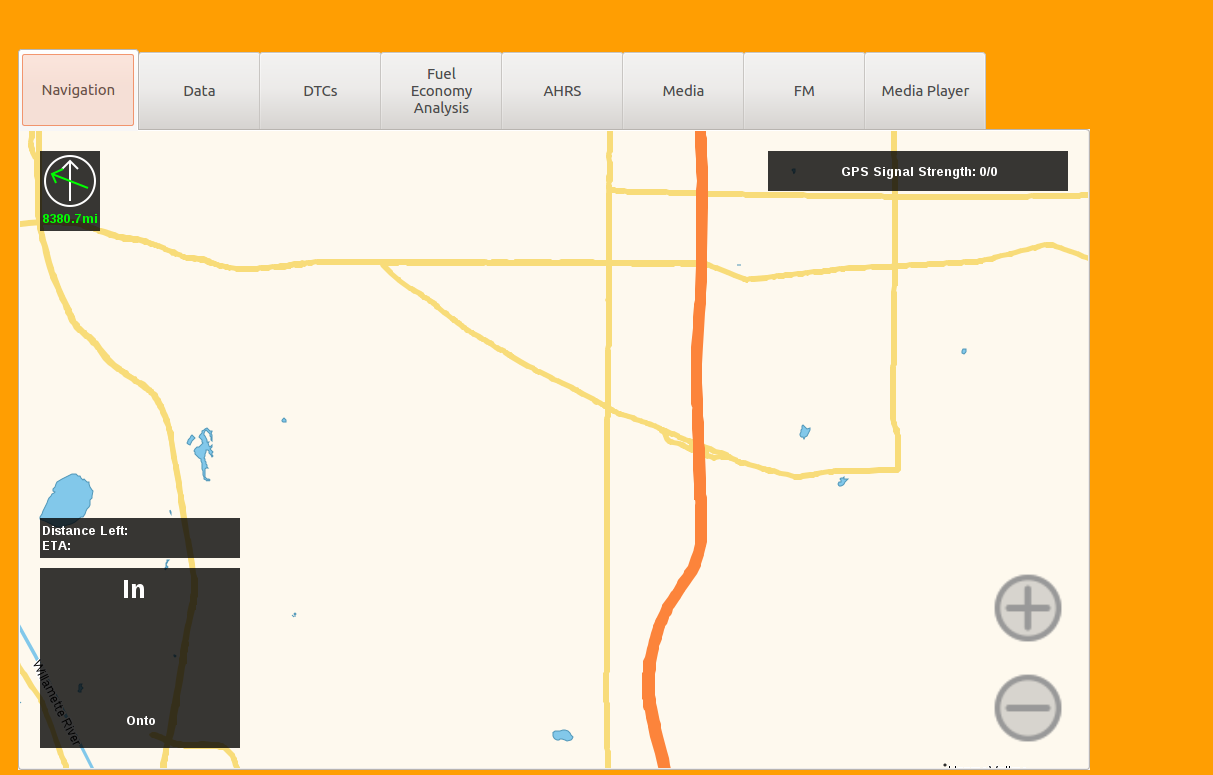
\includegraphics[width=0.85\textwidth]{nav.eps}
\centering
\caption{Finalized and integrated navigation screen; GPS sensor is not connected for the screen capture, hence incorrect heading and directional data.}
\end{figure}

\begin{figure}[h]
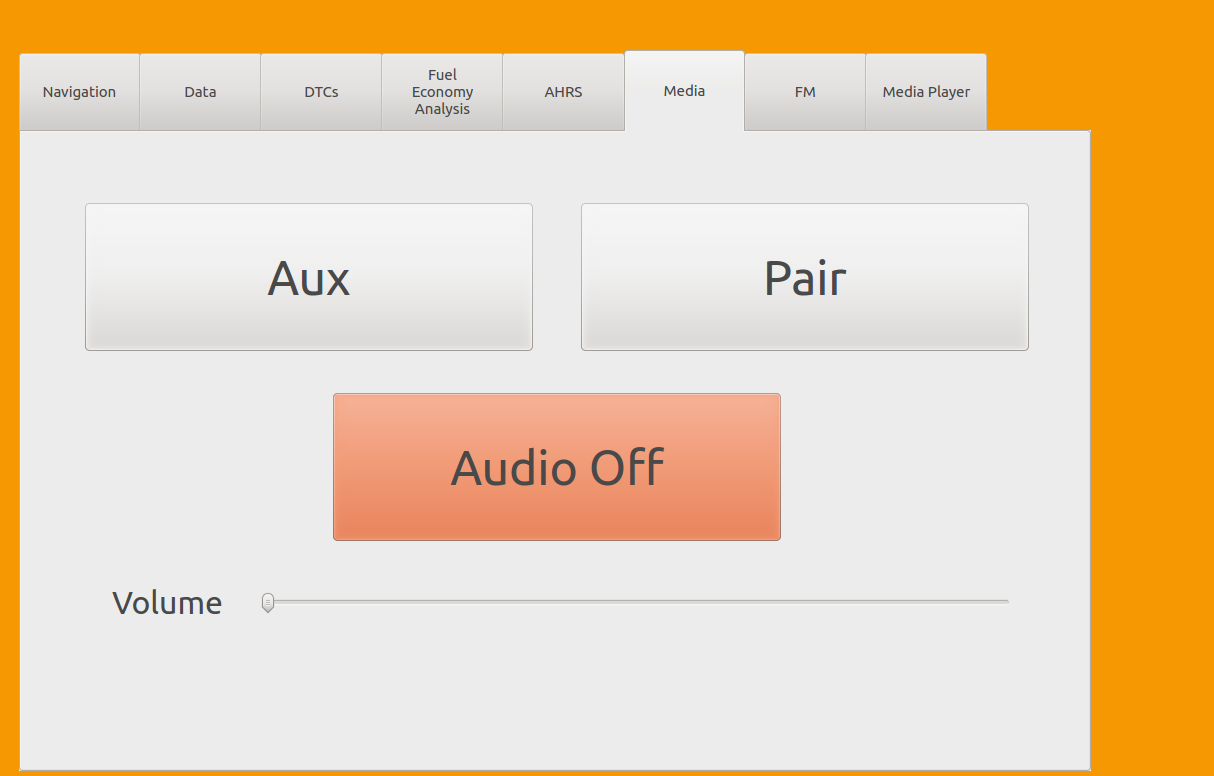
\includegraphics[width=0.85\textwidth]{media.eps}
\centering
\caption{Media menu with options for auxiliary input and bluetooth streaming.}
\end{figure}

\begin{figure}[h]
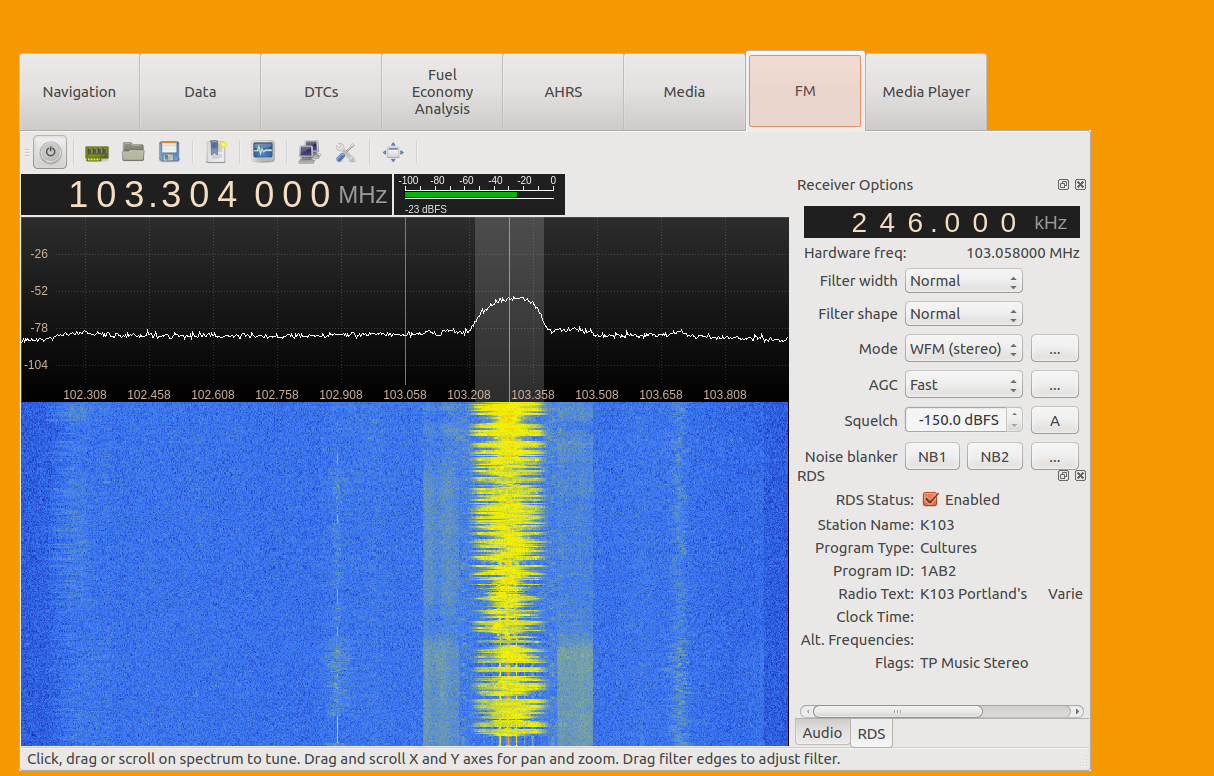
\includegraphics[width=0.85\textwidth]{radio.eps}
\centering
\caption{Finalized FM radio with RDS information.}
\end{figure}

\end{document}
